\documentclass{beamer}
\usepackage{beamerthemeshadow}
\usepackage{color}
%\usepackage[all]{xy}


%%%% choose your presentation style:
\mode<presentation>
{
  \usetheme{Copenhagen} %%%
 \usecolortheme{beaver}

%%% set style for ovelays: lists (and other text) appearing one item at a time
%%% This will create a dimmed preview of next item:
\setbeamercovered{transparent}
%%% This will hide it entirely:
%\setbeamercovered{invisible}
}
%% if you don't want page numbers to show: 
\setbeamertemplate{footline}[page number]{}


\begin{document}
\title{Parallel BVH Construction for Real-Time Ray Tracing}
\author{Aaron Lemmon}
\institute[UMM] % (optional, but mostly needed)
{
 % \inst{1}%
  University of Minnesota, Morris
}
\date[]  
{April 30, 2015}

\begin{frame}
  \titlepage
\end{frame}

\begin{frame}

  \frametitle{Outline}
\tableofcontents
\end{frame}

\section{Bounding Volume Hierarchies}

\begin{frame}
  \frametitle{BVH Example}
\begin{figure}
%%% note: the file is in the same folder as your .tex file
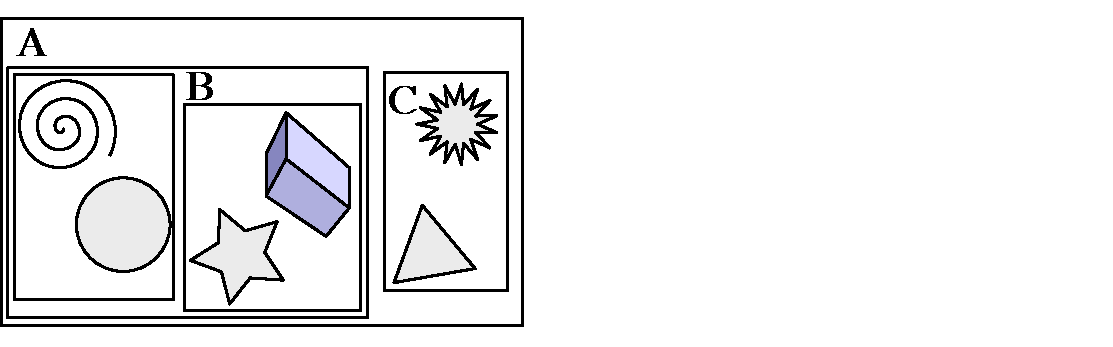
\includegraphics[height=30mm]{bvh_diagram.pdf}
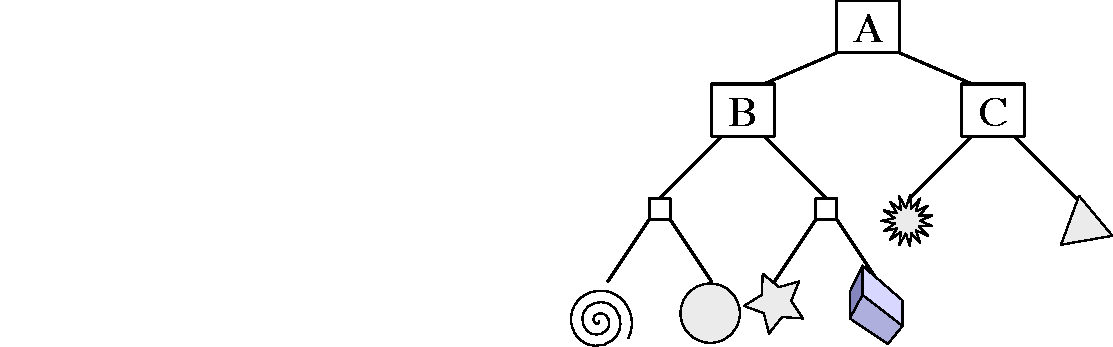
\includegraphics[height=30mm]{bvh_tree.pdf}
\end{figure}
\end{frame}

\section{Z-order Curves}

\begin{frame}
  \frametitle{Morton Codes}
\begin{columns}[t]

\column{.5\textwidth}
\centering
\begin{itemize}
\item Interleave binary representations of coordinate values
\item Transforms multidimensional coordinates into a single value
\item Morton Code contains location information
\item Used to sort objects
\end{itemize}

\column{.5\textwidth}
\begin{figure}
%%% note: the file is in the same folder as your .tex file
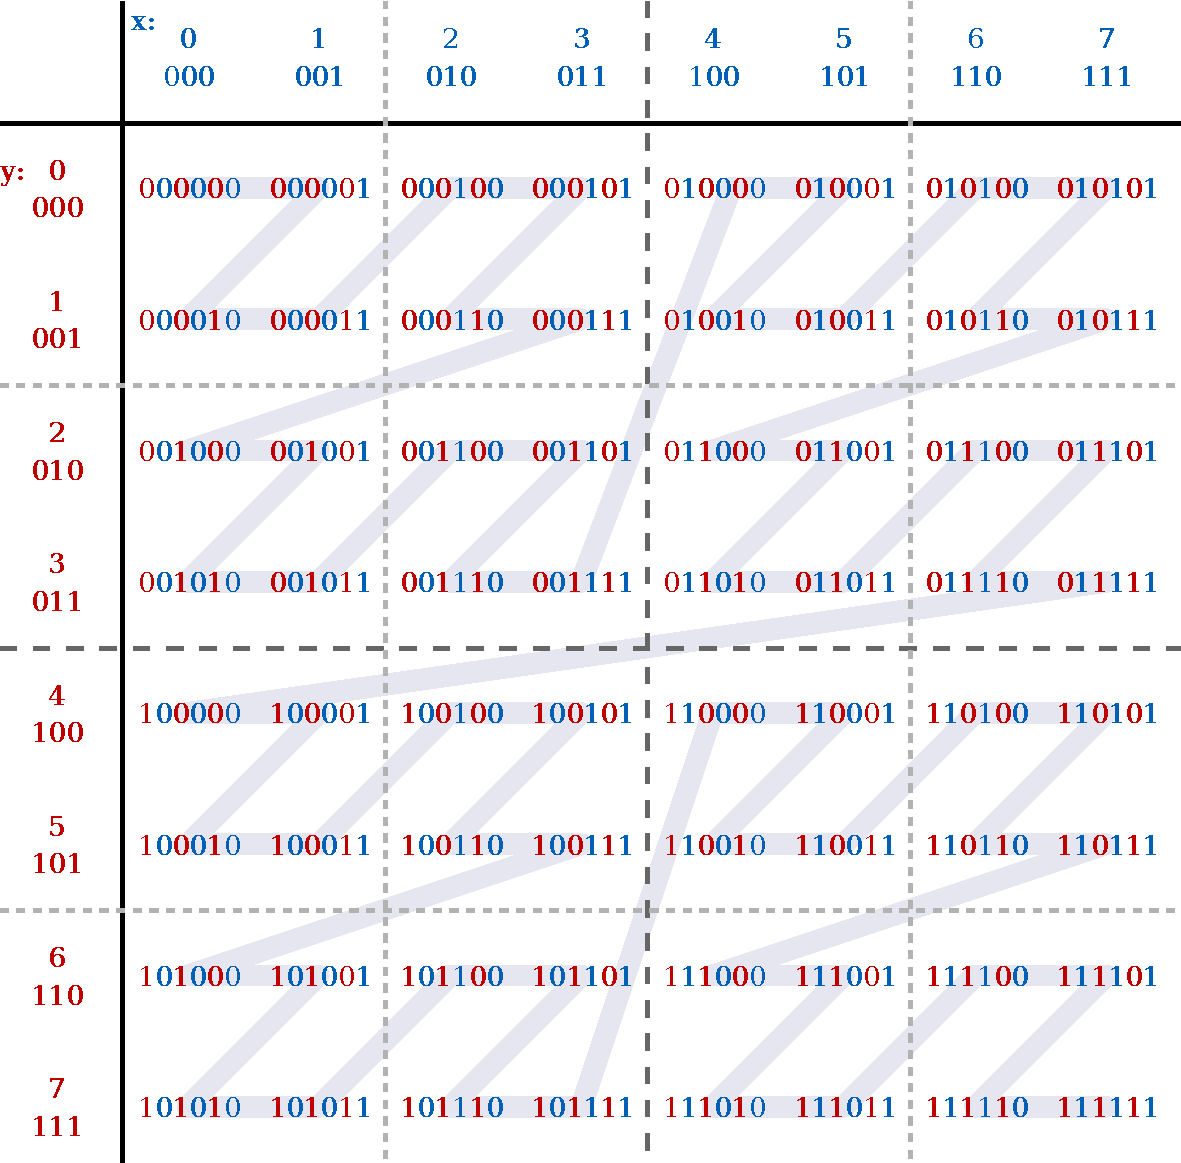
\includegraphics[height=45mm]{Z-curve.pdf}
\end{figure}
\end{columns}
\end{frame}

\begin{frame}
  \frametitle{Shape of a Z-order Curve}
\begin{figure}
%%% note: the file is in the same folder as your .tex file
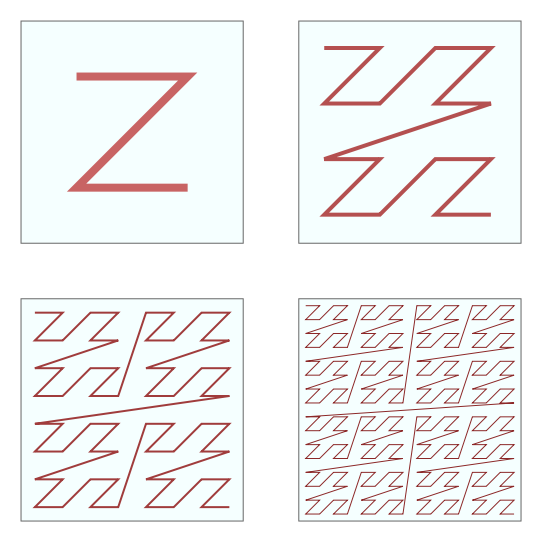
\includegraphics[height=45mm]{542px-Four-level_Z.png}
\end{figure}
\end{frame}

\section{Binary Radix Trees}

\begin{frame}
  \frametitle{Binary Radix Tree Example}
  
\begin{columns}[t]

\column{.5\textwidth}
\begin{figure}
%%% note: the file is in the same folder as your .tex file
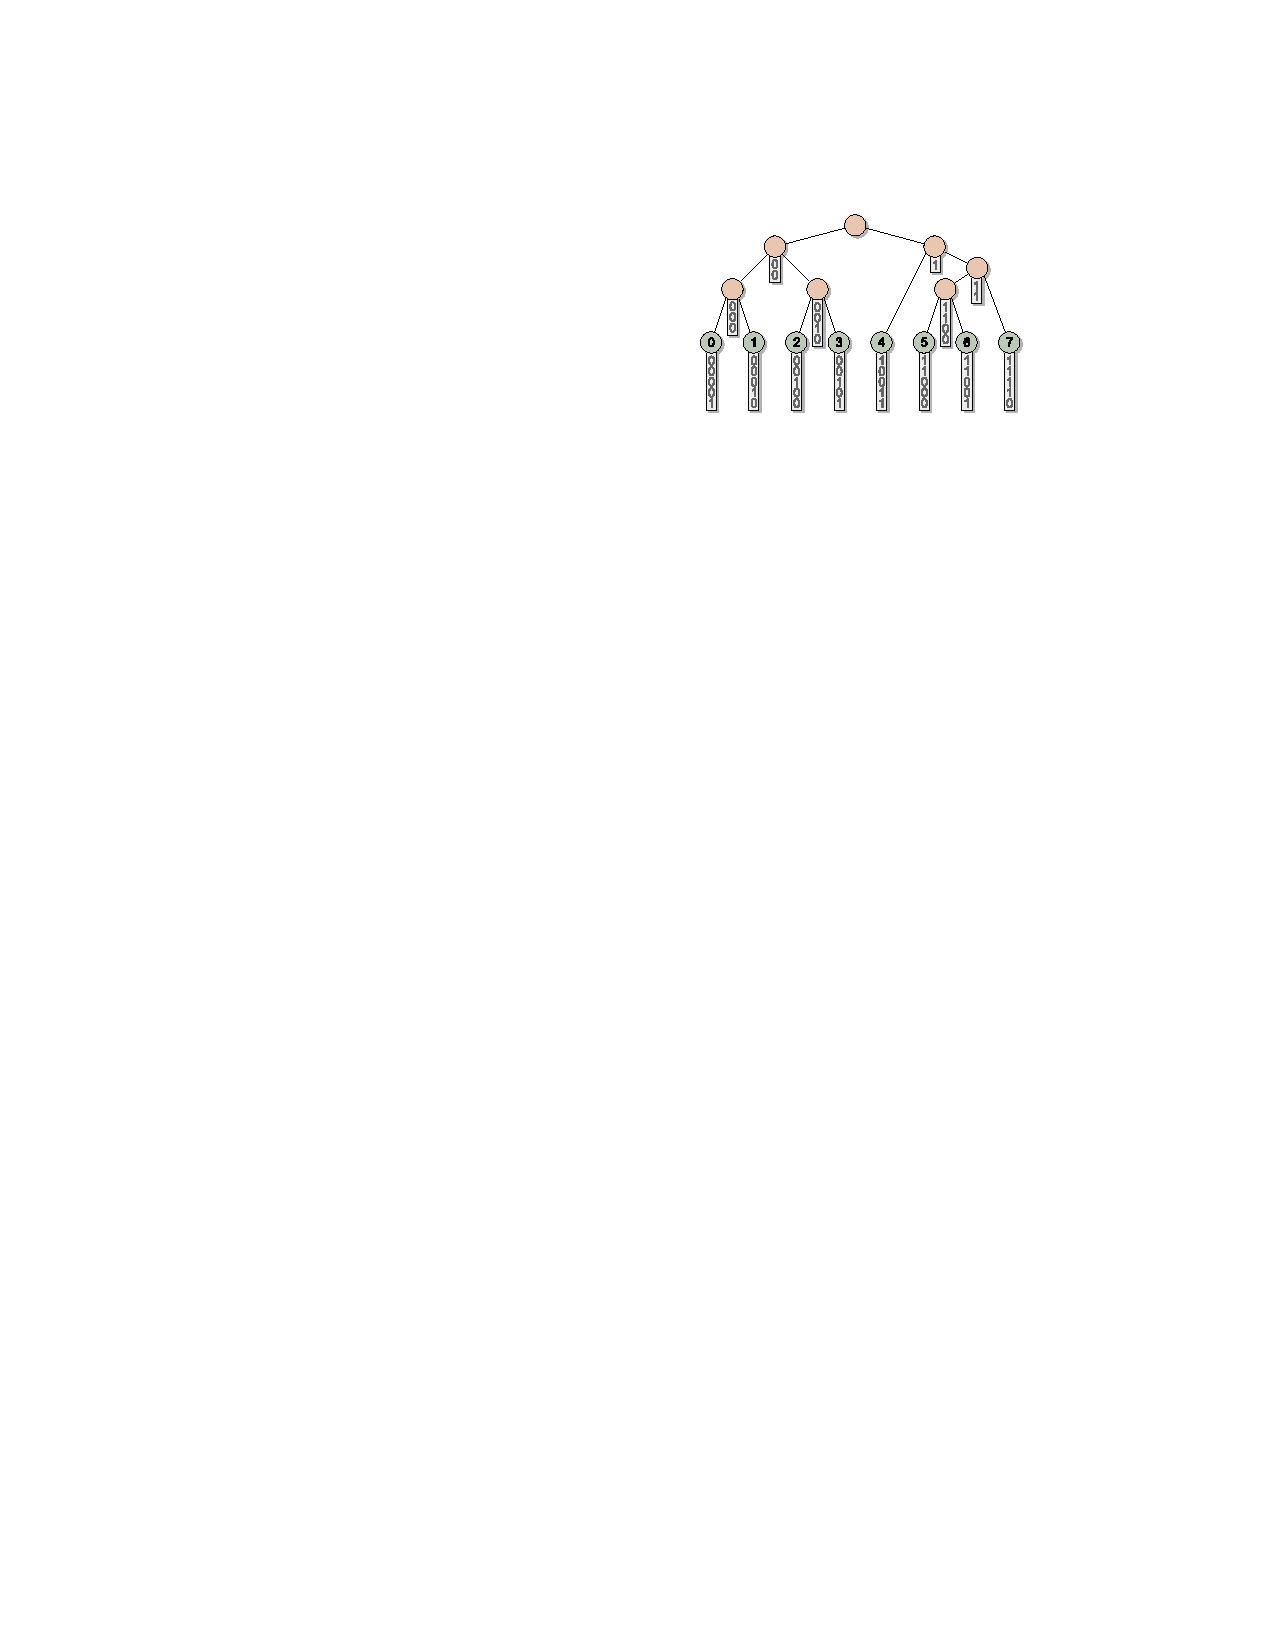
\includegraphics[height=40mm]{BinaryRadixTree.pdf}
\end{figure}

\column{.5\textwidth}
\begin{figure}
%%% note: the file is in the same folder as your .tex file
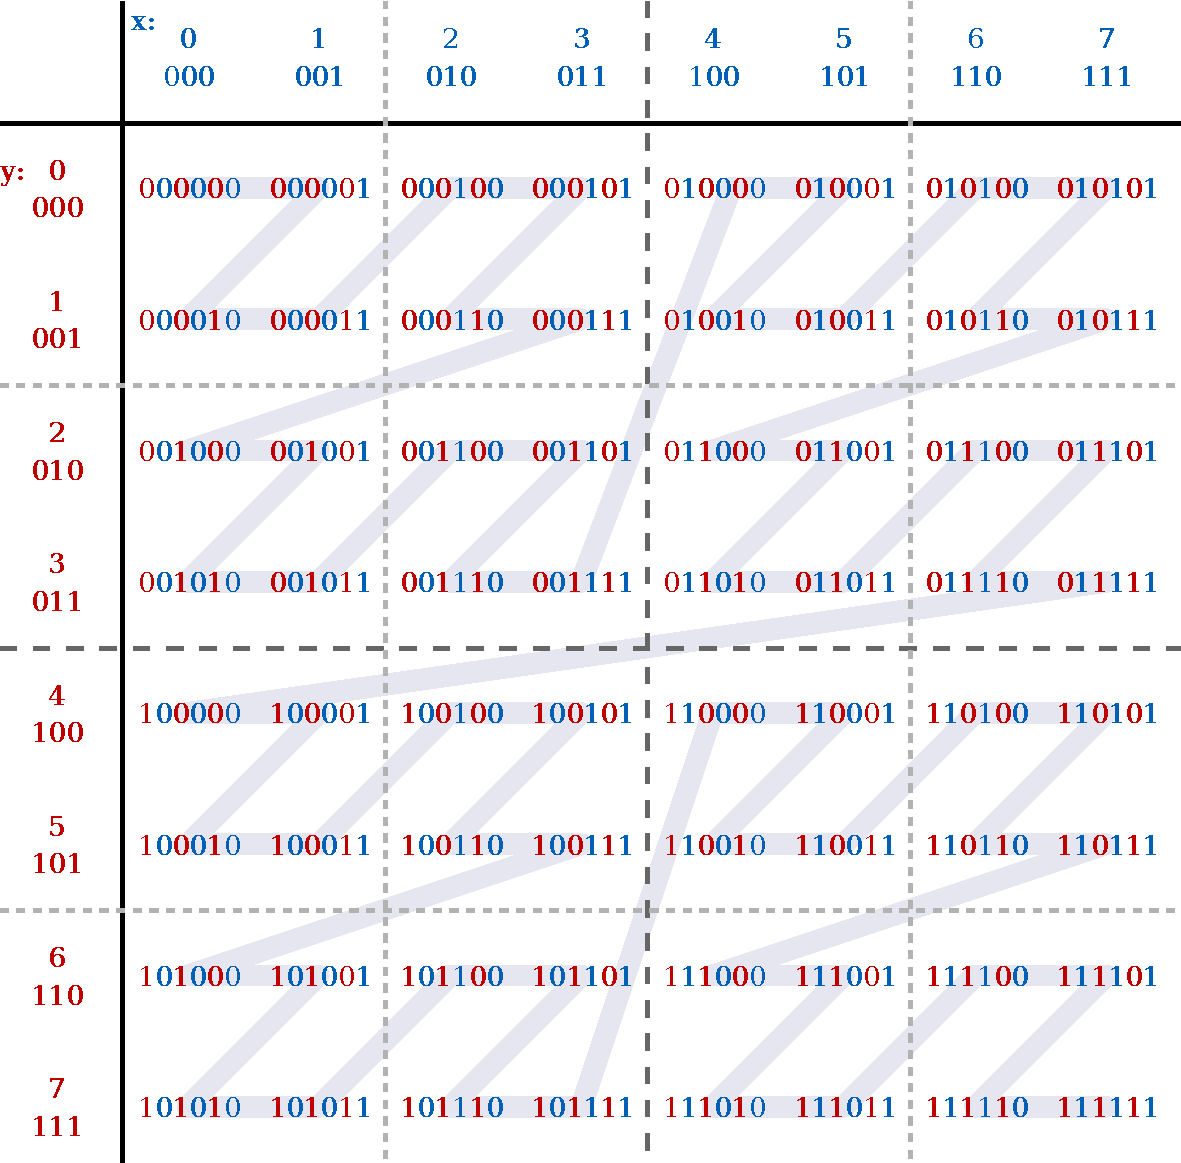
\includegraphics[height=40mm]{Z-curve.pdf}
\end{figure}
\end{columns}
\end{frame}

\begin{frame}
  \frametitle{Discussion}
Questions?
\end{frame}

\end{document}
